% ---------------------------------------------------------------
\section{Introduction}
\slides{1--2}

Opening framing, from the title and ``Main Points'' slides.

\begin{itemize}
    \item Problem: training a robust robotics model from only two to three hours of real egocentric data. Every object, surface and lighting case cannot feasibly be recorded.
    \item Proposal: use the NVIDIA Cosmos family of world foundation models to scale a limited dataset by generating appearance variants of recorded clips.
    \item Three claims the paper will support:
    \begin{enumerate}
        \item A multi-model pipeline on NVIDIA Cosmos can turn a small real dataset into thousands of synthetic training clips.
        \item Changing appearance works for simpler scenes. Complex scenes and action-level changes remain unsolved.
        \item Structured reasoning about a scene produces better variations than random augmentation.
    \end{enumerate}
    \item The open question that frames the paper: is synthetic appearance data enough to make a robot more robust, or does action generation have to be solved first?
\end{itemize}

\paragraph{Contributions, as the deck states them.} Pipeline (Sec.~\ref{sec:pipeline}); ontology-driven variation and prompt principles (Sec.~\ref{sec:part1}); multi-map guidance and mask construction (Sec.~\ref{sec:part2}); qualitative results and their boundary (Sec.~\ref{sec:results}); a path to closing the gap (Sec.~\ref{sec:future}).

% ---------------------------------------------------------------
\section{What We Started With and What We Created}
\label{sec:startend}
\slides{3--4}

\begin{figure}[htbp]
\centering
\begin{subfigure}{0.49\linewidth}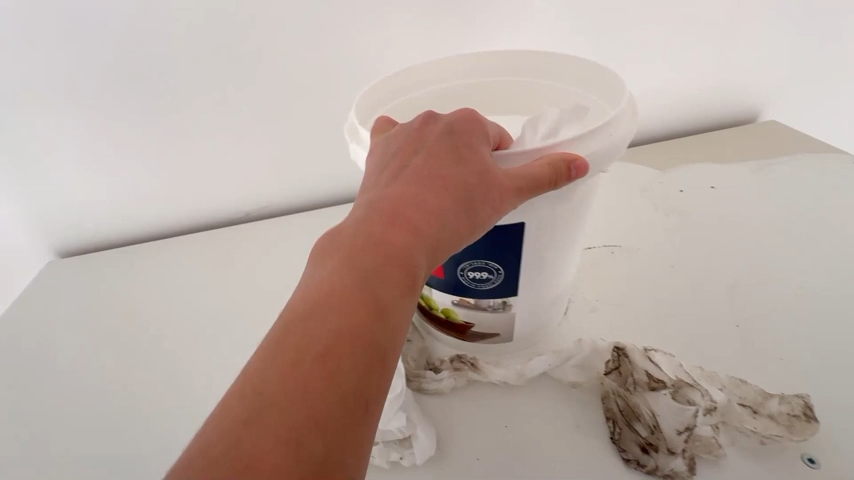
\includegraphics[width=\linewidth]{s03_original.png}\caption{What we started with}\end{subfigure}\hfill
\begin{subfigure}{0.49\linewidth}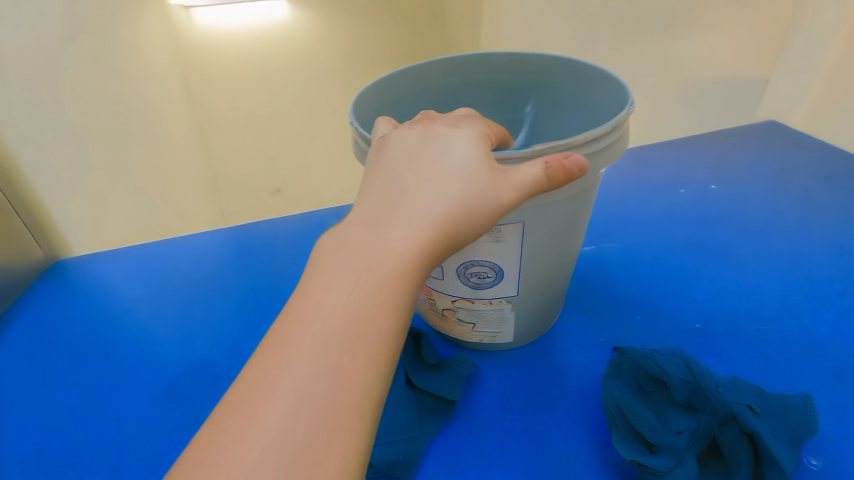
\includegraphics[width=\linewidth]{s04_created.png}\caption{What we created}\end{subfigure}
\caption{The running example. (a) A person wiping down a table with a bucket and a rag, one of the real clips. (b) The variant produced by the pipeline when asked to change only the countertop to blue. The wall color has changed completely, and blue has bled into the rag.}
\label{fig:startend}
\end{figure}

\begin{itemize}
    \item The source clip (Fig.~\ref{fig:startend}a): a person wiping a table with a bucket and a rag. Is this one scene enough to train a robust policy? A robot trained only on it might fail the moment the surface color changes or the bucket is swapped.
    \item Goal: scale this one clip through permutations of the objects and actions observed.
    \item The variant (Fig.~\ref{fig:startend}b): produced from the same clip by the pipeline, targeting only the countertop color. The model struggles in places: the wall color changed completely and the blue bled into the rag. Sections~\ref{sec:part2} and~\ref{sec:results} say where and why.
    \item Key point: from one version of the scene to a plausible variation without recording new video.
\end{itemize}

% ---------------------------------------------------------------
\section{Background: NVIDIA Cosmos}
\label{sec:cosmos}
\slides{5}

\begin{itemize}
    \item World foundation models (WFMs) are trained on large volumes of real video to model physics, geometry and causality, and to generate physically plausible future states; NVIDIA positions them as simulators that let robots and autonomous vehicles test outcomes before acting~\cite{cosmos2025}.
    \item \textbf{Cosmos Predict}~\cite{cosmospredict2}: generates future world states as video from text, image or video input (Text2World, Image2World, Video2World); 2B and 14B parameter scales.
    \item \textbf{Cosmos Transfer}~\cite{cosmostransfer1,cosmostransfer25}: adapts video across environments, lighting and domains (Sim2Real, Real2Real) with multi-control conditioning on depth, segmentation and edge maps. Primarily used here for aesthetic transformations.
    \item \textbf{Cosmos Reason}~\cite{cosmosreason1}: vision-language model for physical scene understanding; reasons over objects, intent and interactions with chain-of-thought; annotates and critiques synthetic data.
    \item Cosmos~3 (2026) unifies Predict, Transfer and Reason in a single omni-model built on a Mixture-of-Transformers architecture~\cite{cosmos3}.
    \item This work uses Transfer and Reason.
\end{itemize}

% ---------------------------------------------------------------
\section{How We Used World Foundation Models}
\label{sec:pipeline}
\slides{6}

\begin{figure}[htbp]
\centering
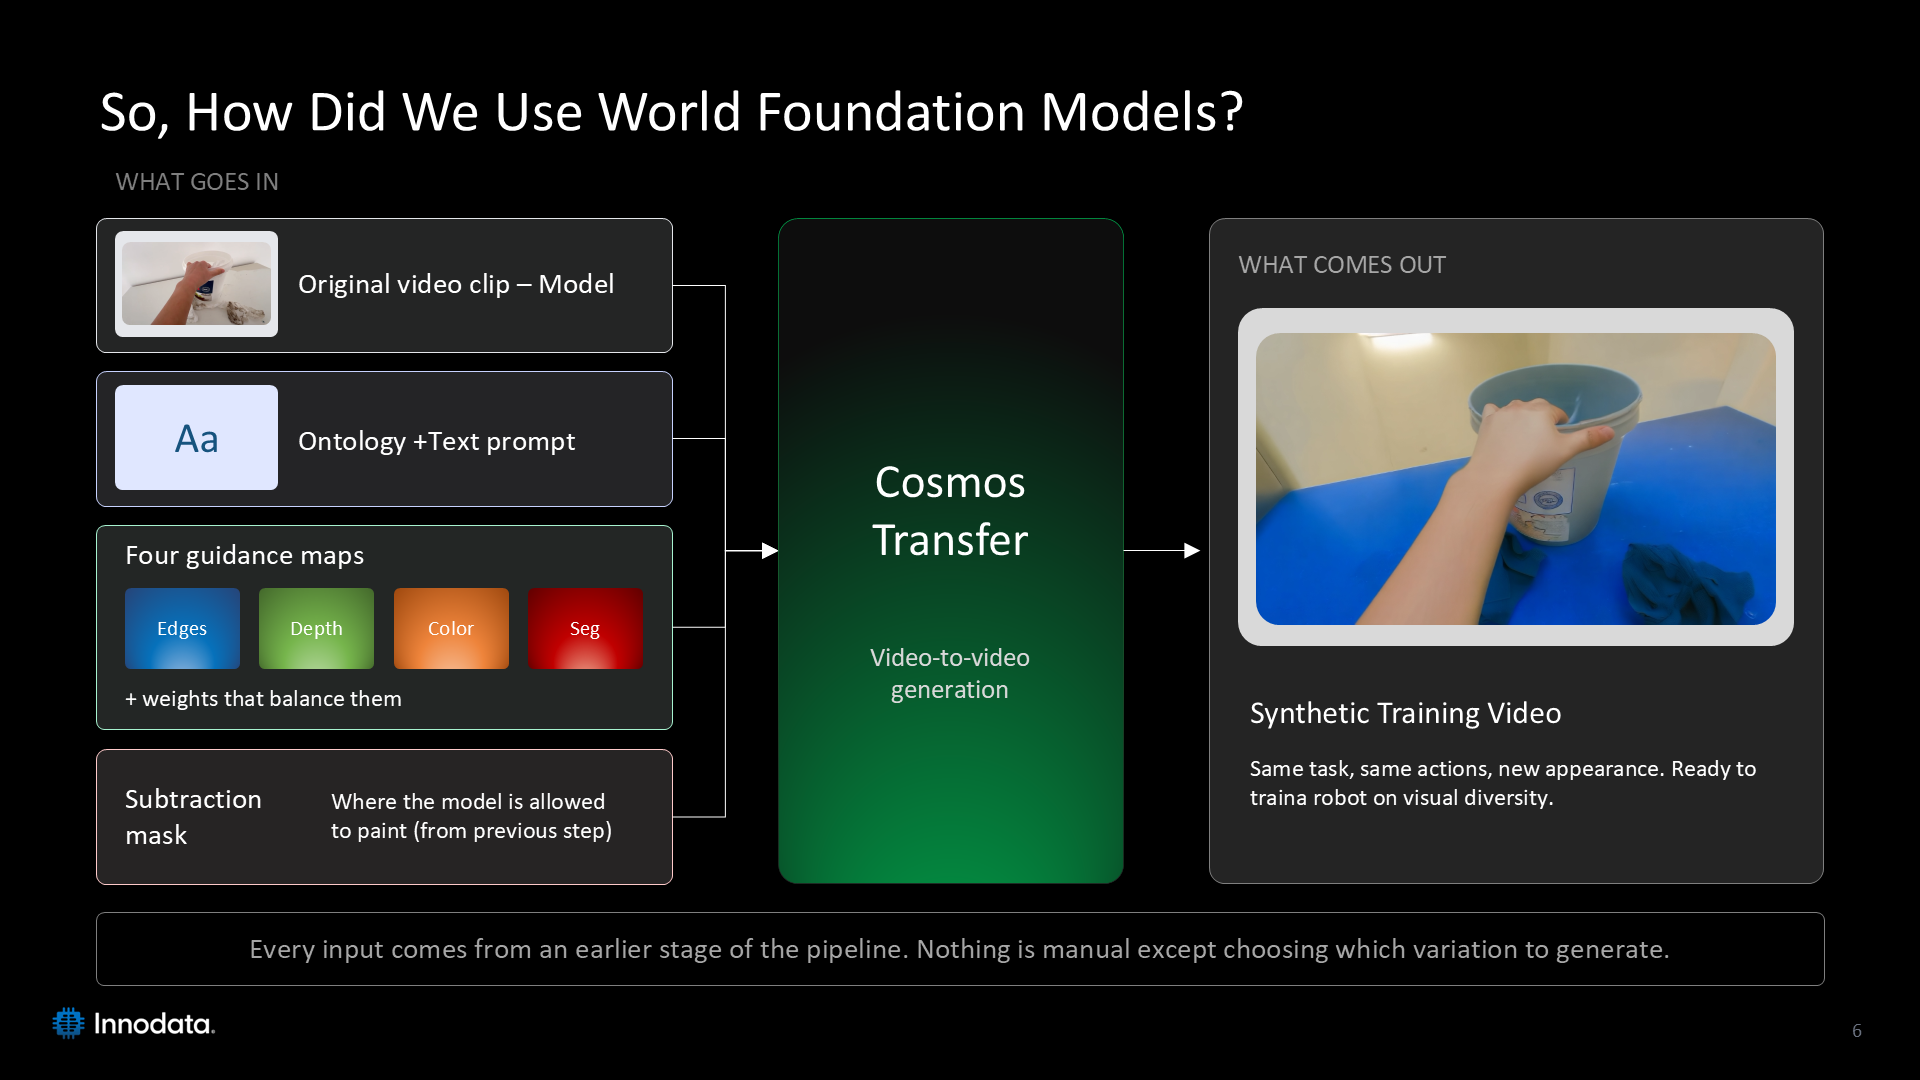
\includegraphics[width=\linewidth]{slide06_pipeline.png}
\caption{Pipeline as presented. Inputs on the left: the original clip, the ontology and text prompt, four guidance maps with balancing weights, and a subtraction mask marking where the model may paint. Cosmos Transfer performs video-to-video generation. Output on the right: a synthetic training video with the same task and actions and a new appearance. (Redraw as a vector figure for the final version.)}
\label{fig:pipeline}
\end{figure}

\begin{itemize}
    \item Original clip prepared with Cosmos Curate.
    \item The clip is fed to Cosmos Reason, which produces an ontology, a structured understanding of the observed scene (Sec.~\ref{sec:ontology}).
    \item The ontology goes to GPT-4o mini, which writes the text prompt in the form Cosmos Transfer expects (Sec.~\ref{sec:prompts}).
    \item Four guidance maps are generated to preserve edges, depth and color, plus a segmentation; a subtraction mask restricts where the model may paint (Sec.~\ref{sec:part2}).
    \item Cosmos Transfer renders the synthetic training video: same task, same actions, new appearance.
    \item Every input comes from an earlier stage of the pipeline. Nothing is manual except choosing which variation to generate.
\end{itemize}

% ---------------------------------------------------------------
\section{Part 1: Reasoning with Structured Ontologies}
\label{sec:part1}

\subsection{Ontology-driven variation}
\slides{7}

\begin{itemize}
    \item Premise: the model must associate objects with the actions and physical context they take part in, not just with how they look.
    \item Contrast with domain randomization~\cite{tobin2017}, the standard technique in robotics: colors, textures and lighting are swapped at random in the hope that the policy learns to generalize, with no understanding of the scene.
    \item Ontology-driven variation instead:
    \begin{itemize}
        \item understands the scene first: objects, states, materials, actions, lighting;
        \item links each object to its role in the task, so that a bucket in a cleaning task is a cleaning bucket, which behaves differently from a bucket on a shelf;
        \item proposes only physically grounded variations per object;
        \item is structured, auditable and filterable.
    \end{itemize}
    \item Result: about 70 plausible variation candidates per 15-second clip, filtered from more than 100 raw proposals.
\end{itemize}

\subsection{Ontology structure: what Cosmos Reason produces}
\label{sec:ontology}
\slides{8}

\begin{figure}[htbp]
\centering
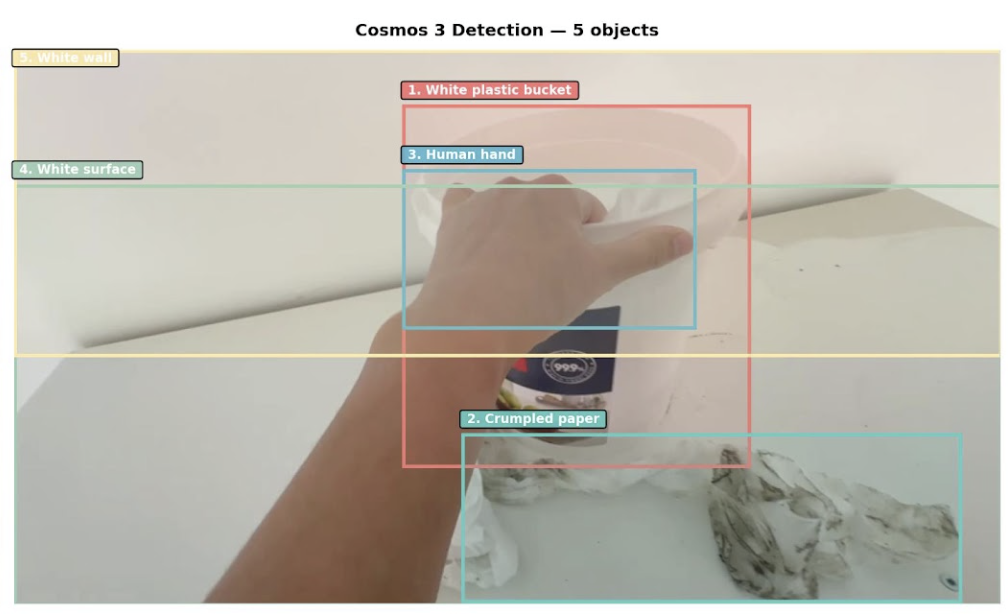
\includegraphics[width=0.75\linewidth]{s08_detection.png}
\caption{Detections for the running example: five task-relevant objects with bounding boxes (white wall, white plastic bucket, crumpled paper, human hand, white surface).}
\label{fig:detection}
\end{figure}

\begin{itemize}
    \item Beyond detection: the ontology records state, material and color for each object and proposes variations grounded in the physical context of the task (Fig.~\ref{fig:detection}).
    \item Excerpt of the ontology for the running example:
\end{itemize}

\begin{lstlisting}
"task": {
  "name": "Disposing of crumpled paper into a bucket",
  "phase": "Preparation",
  "action_primitive": "Holding a bucket and positioning it"
},
"key_objects": [{
  "name": "White plastic bucket",
  "role_in_task": "Container for disposing of waste",
  "robustness_gaps": {
    "what_robot_must_handle": ["Different bucket sizes and shapes",
      "Labels with varying colors and designs", "Wet or slippery buckets"],
    "common_failure_modes": ["Bucket slips from hand", "Bucket tips over",
      "Bucket cannot be opened"]
  }
}]
\end{lstlisting}

\begin{itemize}
    \item The model identifies robustness gaps and failure modes such as the bucket tipping over. These are action-level variations, better suited to Cosmos Predict.
    \item It also proposes appearance variations, such as buckets of different colors, designs, sizes and shapes, which suit Cosmos Transfer.
\end{itemize}

\subsection{From ontology to generation-ready prompts}
\label{sec:prompts}
\slides{9}

\begin{itemize}
    \item Input to GPT-4o mini, for the running example: target ``white surface being cleaned''; variation ``change color to solid blue matte''; preserve bucket, cloth, hands, lighting; context: cleaning task, laminate surface, bright overhead lighting.
    \item Output, the Cosmos Transfer prompt: \emph{``The video captures a person cleaning a solid blue countertop in a well-lit indoor kitchen. The countertop surface is a rich, vivid blue color with a smooth matte finish. The bucket and paper towels retain their original appearance\ldots''}
    \item Three prompt-engineering principles discovered by experiment:
    \begin{enumerate}
        \item \textbf{Repeat target attributes.} ``solid blue countertop'' \ldots\ ``vivid blue color'' \ldots\ ``blue countertop surface'': threefold reinforcement.
        \item \textbf{Explicitly preserve unchanged elements.} ``Bucket and paper towels retain their original appearance'' protects non-target objects.
        \item \textbf{Describe the result, not the change.} ``A person cleaning a solid blue countertop,'' not ``change white to blue.''
    \end{enumerate}
    \item GPT-4o mini also acts as a filter, rejecting physically implausible variations before they reach Cosmos Transfer.
\end{itemize}

% ---------------------------------------------------------------
\section{Part 2: How We Guide the Model}
\label{sec:part2}

\subsection{Four maps, four kinds of protection}
\slides{10}

\begin{figure}[htbp]
\centering
\begin{subfigure}{0.24\linewidth}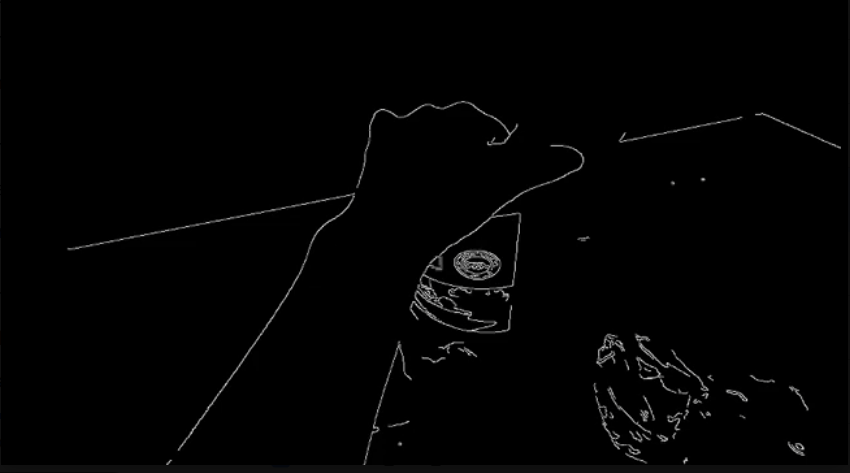
\includegraphics[width=\linewidth]{s10_edges.png}\caption{Edges}\end{subfigure}\hfill
\begin{subfigure}{0.24\linewidth}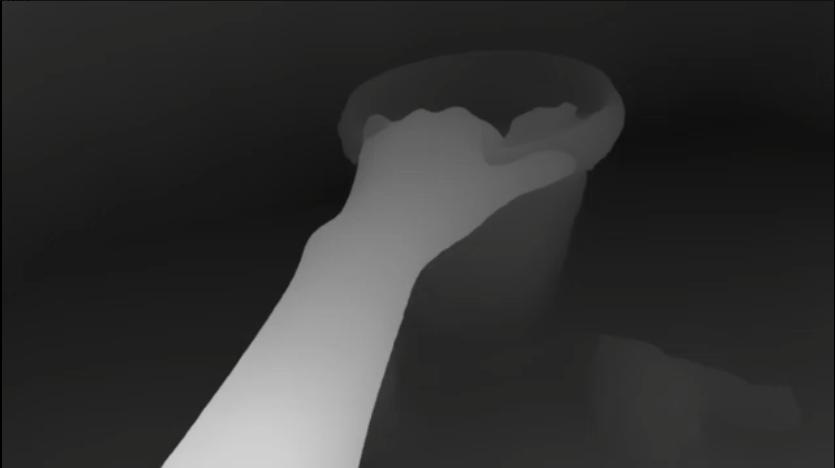
\includegraphics[width=\linewidth]{s10_depth.png}\caption{Depth}\end{subfigure}\hfill
\begin{subfigure}{0.24\linewidth}
\includegraphics[width=\linewidth]{s10_color.png}\caption{Color}\end{subfigure}\hfill
\begin{subfigure}{0.24\linewidth}
\includegraphics[width=\linewidth]{s10_mask.png}\caption{Mask}\end{subfigure}
\caption{The four guidance maps for one frame of the running example. Edges keep the shapes; depth keeps the layout; color keeps the lighting; the mask says where to paint.}
\label{fig:maps}
\end{figure}

\begin{itemize}
    \item The model receives four maps with different weights, each protecting a different part of the original video (Fig.~\ref{fig:maps}).
    \item \textbf{Edges}, ``keep the shapes'': protects the outline of every object in the frame, so the bucket stays a bucket.
    \item \textbf{Depth}, ``keep the layout'': protects what is in front and what is behind, so nothing floats or sinks into the surface.
    \item \textbf{Color}, ``keep the lighting'': protects the overall palette and light direction, so it still looks like the same room.
    \item \textbf{Mask}, ``paint only here'': specifies exactly which pixels the model may change. Think of painter's tape.
    \item The first three maps are generated automatically. The mask needs one extra step.
\end{itemize}

\subsection{Tuning the maps and building the mask}
\slides{11}

\begin{figure}[htbp]
\centering
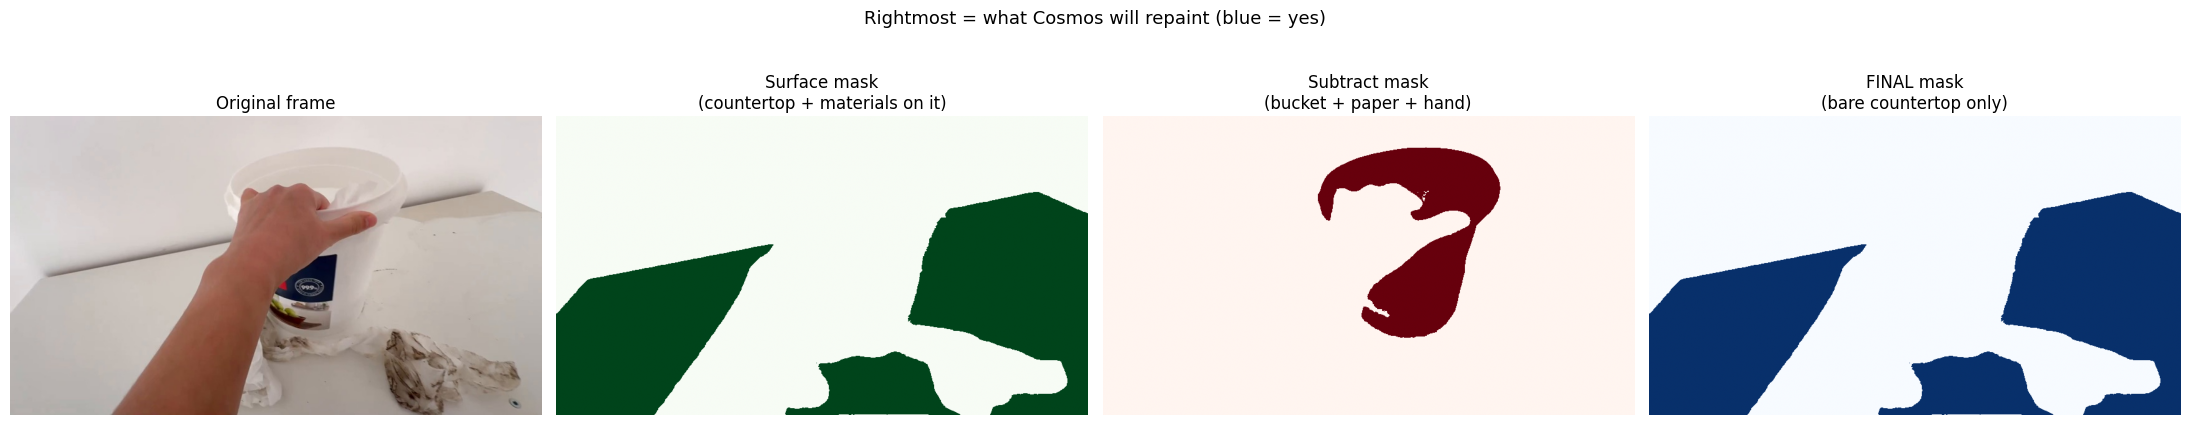
\includegraphics[width=\linewidth]{s11_mask_strip.png}
\caption{Building the subtraction mask. Left to right: original frame; surface mask (countertop plus the materials on it); subtract mask (bucket, paper and hand); final mask (bare countertop only). Blue marks what Cosmos will repaint.}
\label{fig:maskstrip}
\end{figure}

What we learned from tuning:
\begin{itemize}
    \item \textbf{Edges matter most.} Too high and nothing changes; too low and objects warp.
    \item \textbf{Color guidance must be nearly off.} If the goal is to repaint something, this map fights the change.
    \item \textbf{Prompt strength controls boldness.} Higher settings give the model more confidence to commit.
\end{itemize}

How the mask is built (Fig.~\ref{fig:maskstrip}). The countertop and the bucket overlap; to change one without the other:
\begin{enumerate}
    \item find the surface;
    \item find what is on it;
    \item subtract;
    \item use the result as the final mask.
\end{enumerate}
The bounding boxes come from the same scene model that built the ontology. No extra tools are needed.

% ---------------------------------------------------------------
\section{Results}
\label{sec:results}
\slides{12--16}

\subsection{Simple aesthetic variations}
\slides{13}

\begin{figure}[htbp]
\centering
\begin{subfigure}{0.49\linewidth}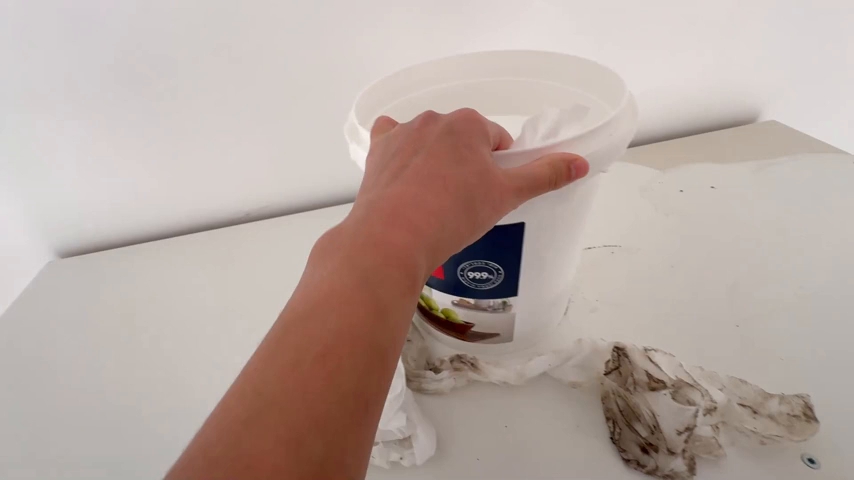
\includegraphics[width=\linewidth]{s13_old.png}\caption{Old}\end{subfigure}\hfill
\begin{subfigure}{0.49\linewidth}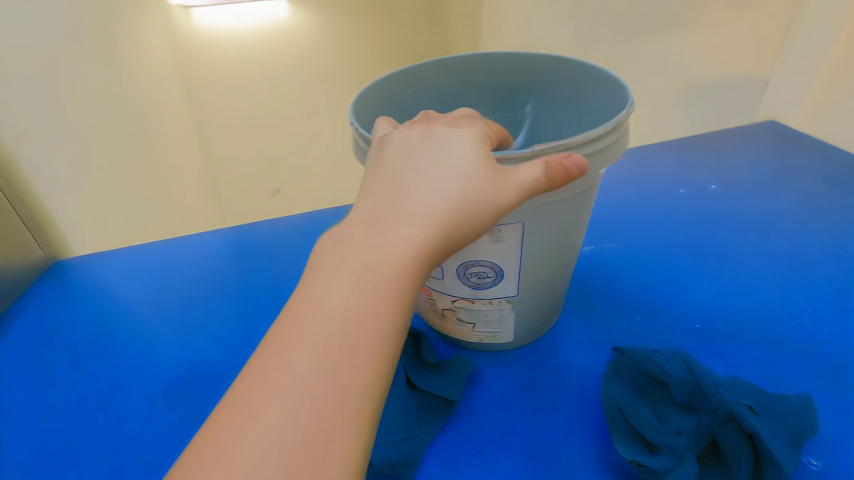
\includegraphics[width=\linewidth]{s13_new.png}\caption{New}\end{subfigure}
\caption{The models perform simple aesthetic variations fairly well: the countertop is recolored while the hand pose, bucket geometry and motion are retained.}
\label{fig:simple}
\end{figure}

\begin{itemize}
    \item The models handle simple aesthetic variations fairly well (Fig.~\ref{fig:simple}).
    \item To note in the text: the same output also shows the leakage described in Sec.~\ref{sec:startend} (wall, rag and bucket tone), which is the boundary explored next.
\end{itemize}

\subsection{Multi-texture scenes}
\slides{14}

\begin{figure}[htbp]
\centering
\begin{subfigure}{0.49\linewidth}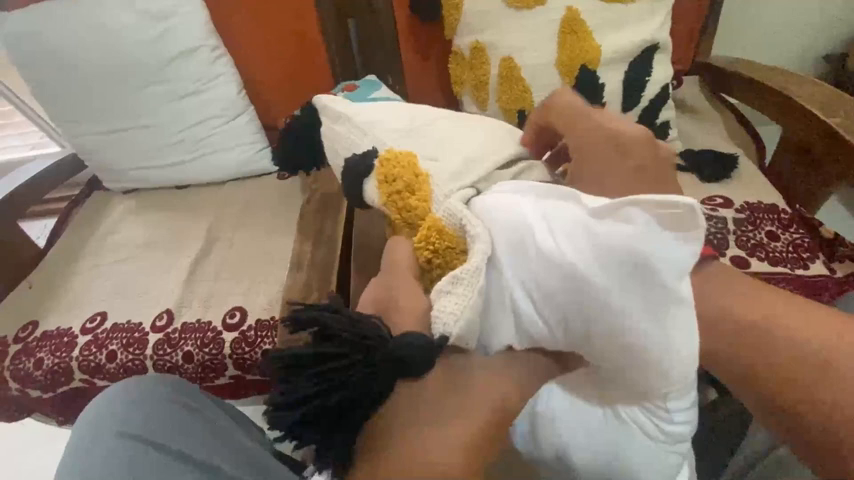
\includegraphics[width=\linewidth]{s14_old.png}\caption{Old}\end{subfigure}\hfill
\begin{subfigure}{0.49\linewidth}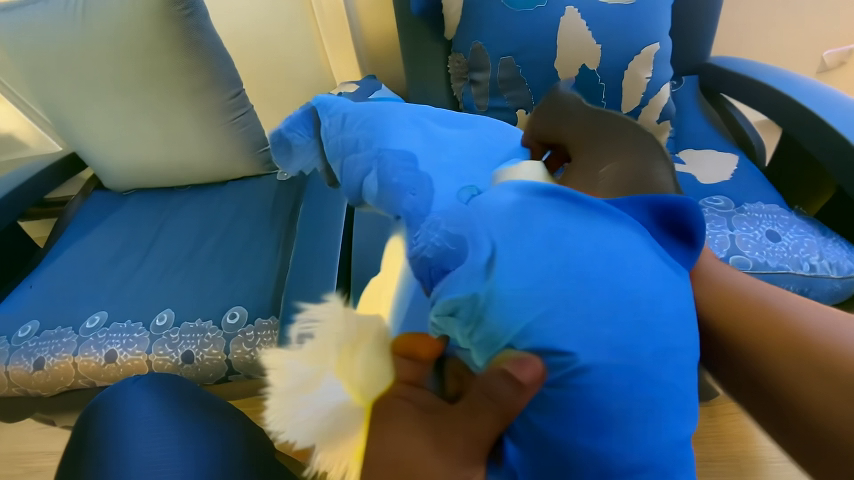
\includegraphics[width=\linewidth]{s14_new.png}\caption{New}\end{subfigure}
\caption{The model struggles heavily with a clip whose frame has multiple textures: nearly every surface is recolored, and the cushion patterns survive only as blue-on-blue relief.}
\label{fig:multitexture}
\end{figure}

\begin{itemize}
    \item The model struggles fairly heavily with a clip like Fig.~\ref{fig:multitexture}, where the frame contains multiple textures.
\end{itemize}

\subsection{A physics-minded task}
\slides{15}

\begin{figure}[htbp]
\centering
\begin{subfigure}[t]{0.28\linewidth}\centering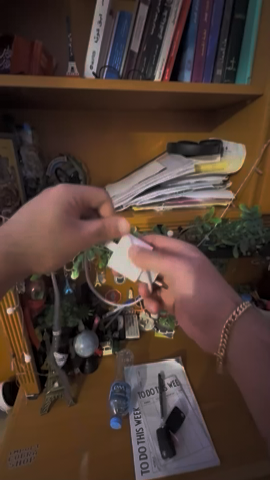
\includegraphics[height=4.2cm]{s15_original.png}\caption{Original}\end{subfigure}\hfill
\begin{subfigure}[t]{0.68\linewidth}\centering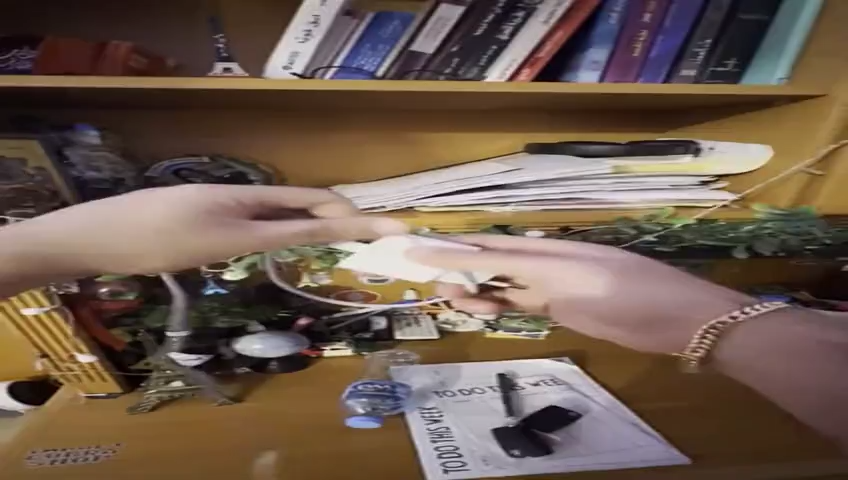
\includegraphics[height=4.2cm]{s15_generated.png}\caption{Generated (Cosmos Predict)}\end{subfigure}
\caption{Physics-minded task: unravel a cord clockwise at constant angular velocity. The generated clip reproduces the scene without performing the motion.}
\label{fig:physics}
\end{figure}

\begin{itemize}
    \item The model was asked to perform a physics-minded task: unravel a cord in a clockwise direction at constant angular velocity (Fig.~\ref{fig:physics}).
    \item This is an action-level variation and was run with Cosmos Predict rather than Transfer.
    \item Outcome: the scene is reproduced; the cord does not move.
\end{itemize}

\subsection{More results}
\slides{16}

\begin{figure}[htbp]
\centering
\begin{subfigure}[t]{0.15\linewidth}\centering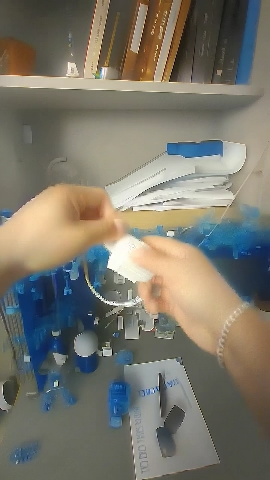
\includegraphics[height=2.7cm]{s16_left.png}\caption{Shelf}\end{subfigure}\hfill
\begin{subfigure}[t]{0.41\linewidth}\centering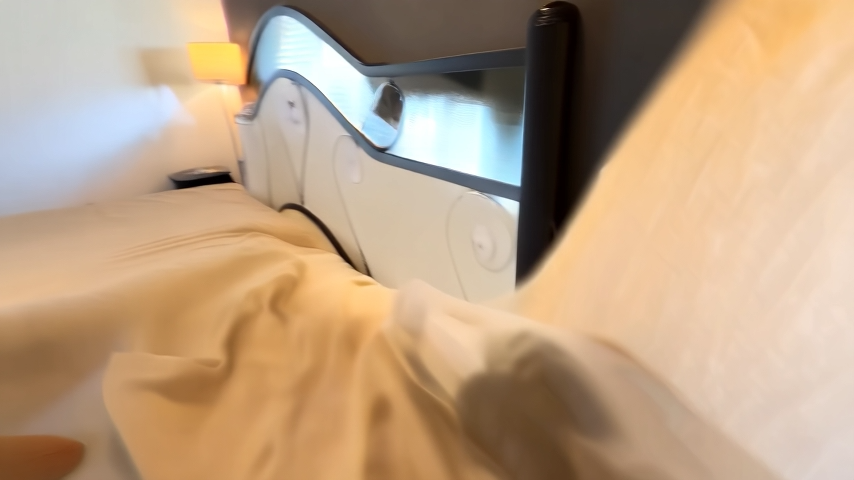
\includegraphics[height=2.7cm]{s16_middle.png}\caption{Bed, rug}\end{subfigure}\hfill
\begin{subfigure}[t]{0.41\linewidth}\centering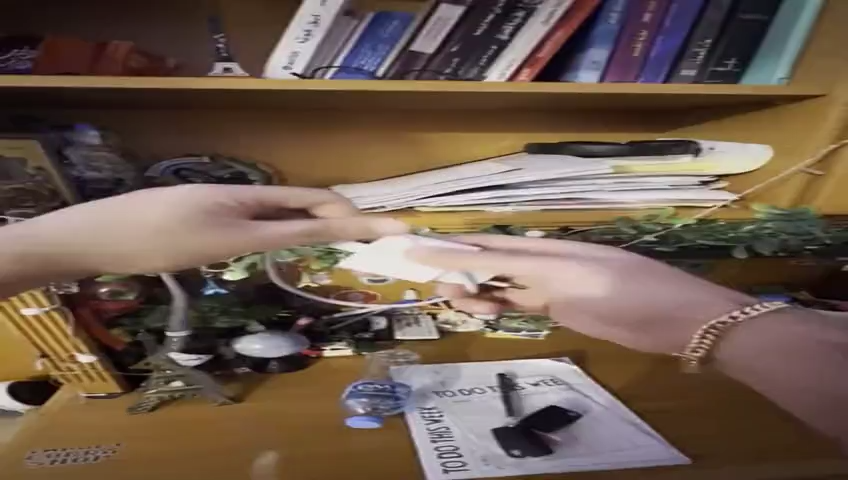
\includegraphics[height=2.7cm]{s16_right.png}\caption{Paper rotation}\end{subfigure}
\caption{Further results. (a) Blue desk-and-shelf variant: color spreads onto shelf objects and the cable. (b) Bed-making clip with a rug texture prompt: surfaces smear and the hand warps. (c) Paper-rotation prompt with Cosmos Predict: no visible change.}
\label{fig:more}
\end{figure}

\begin{itemize}
    \item Three further renders (Fig.~\ref{fig:more}), each showing a distinct failure: color leakage beyond the target, geometric warping, and a no-op on an action prompt.
\end{itemize}

% ---------------------------------------------------------------
\section{Closing the Gap and Future Directions}
\label{sec:future}
\slides{17--18}

Two paths to close the gap:
\begin{itemize}
    \item \textbf{Fine-tuning.} Teach Cosmos Predict the contact physics it lacks by fine-tuning on real manipulation video, with small focused adapters (LoRA) rather than retraining the whole model. If it works, it unlocks action-level synthetic data.
    \item \textbf{Cosmos~3.} The longer-term bet: Cosmos~3 collapses the three-model pipeline into a single architecture with a reasoning tower and a generation tower, with spatial reasoning built into the training data. The Nano 8B version fits on the A100 hardware already in use, but the tooling is very early~\cite{cosmos3,cosmos3nano}.
\end{itemize}

What still needs to be done:
\begin{enumerate}
    \item Scale to more than 100 clips with automated prompt generation.
    \item Test whether appearance-only variations improve policy robustness. Everything so far is qualitative; this is the top priority.
    \item Explore multi-view generation for a richer training signal.
\end{enumerate}

% ---------------------------------------------------------------
\section{Key Takeaways}
\label{sec:takeaways}
\slides{19}

\begin{enumerate}
    \item A multi-model pipeline on NVIDIA Cosmos can turn a small real dataset into thousands of synthetic training clips.
    \item Changing appearance works for simpler scenes. Complex scenes and action-level changes remain unsolved.
    \item Structured reasoning about a scene produces better variations than random augmentation.
\end{enumerate}

The open question: is synthetic appearance data enough to make a robot more robust, or do we need to solve action generation first?

